% !TEX encoding = UTF-8 Unicode
\documentclass[a4paper]{article}

\usepackage{color}
\usepackage{url}
\usepackage[T2A]{fontenc}
\usepackage[utf8]{inputenc}
\usepackage{graphicx}

\usepackage[english,serbian]{babel}

\usepackage[unicode]{hyperref}
\hypersetup{colorlinks,citecolor=green,filecolor=green,linkcolor=blue,urlcolor=blue}

\usepackage{listings}

\newtheorem{primer}{Primer}[section]

\definecolor{mygreen}{rgb}{0,0.6,0}
\definecolor{mygray}{rgb}{0.5,0.5,0.5}
\definecolor{mymauve}{rgb}{0.58,0,0.82}

\lstset{ 
  backgroundcolor=\color{white},
  basicstyle=\scriptsize\ttfamily,
  breakatwhitespace=false,
  breaklines=true,
  captionpos=b,
  commentstyle=\color{mygreen},
  deletekeywords={...},            
  escapeinside={\%*}{*)},          
  extendedchars=true,
  firstnumber=1,              
  frame=single,	                
  keepspaces=true,
  keywordstyle=\color{blue},     
  language=Python,                
  morekeywords={*,...},
  numbers=left, 
  numbersep=5pt,                  
  numberstyle=\tiny\color{mygray}, 
  rulecolor=\color{black},
  showspaces=false,
  showstringspaces=false,
  showtabs=false,
  stepnumber=1, 
  stringstyle=\color{mymauve},
  tabsize=2,
  title=\lstname
}

\begin{document}

\title{F\# na .NET platformi\\ \small{Seminarski rad u okviru kursa\\Metodologija stručnog i naučnog rada\\ Matematički fakultet}}

\author{Tijana Todorov, Tamara Garibović,\\ David Nedeljković, Mihajlo Vićentijević \\ tijana.todorov710@gmail.com, t.garibovic1995@gmail.com, \\ dnedeljkovic710@gmail.com, mihajlovicent@gmail.com}

%\date{9.~april 2015.}

\maketitle

\abstract{
Ovaj rad predstavlja specifičnosti i zanimljivosti o programskom jeziku F\#. U njemu ćete pronaći podatke o njegovom istorijskom poreklu. Zatim, zašto je korisno naučiti ovaj jezik i kakve sve mogućnosti on pruža. Upoznaćete F\# kroz funkcionalno, paralelno i asinhrono programiranje. Možete pročitati zašto je .NET platforma važna za ovaj jezik i kako je ona nastala. Saznaćete kako instalirati i pokrenuti ovaj jezik na Windows i Linux operativnim sistemima. Na {\em Fizz Buzz} problemu predstavljena je ukratko sintaksa jezika F\#. Opisan je mehanizam {\em 'Units of Measure'} koji se u ovom jeziku može koristiti.}

\tableofcontents
\addtocontents{toc}
{\setcounter{tocdepth}{1}}

\newpage

\section{Uvod}
\label{sec:uvod}

F\# je programski jezik koji danas ima veoma široku upotrebu. Pronašao je svoju primenu u raznim oblastima među kojima su i bioinformatika, finansijsko modelovanje, statistika, baze podataka i mnoge druge. Nastao je velikim trudom svog autora, {\em Don Syme}-a, koji je želeo da preusmeri jezike iz familije strogo tipiziranih funkcionalnih jezika na .NET platformu. Ova platforma je razvijena u okviru kompanije {\em Microsoft} i danas ima veoma široku upotrebu. Zahvaljujući tome ovaj jezik je kompatibilan sa svim jezicima koje platforma .NET podržava što pruža jako velike mogućnosti. Jezik je pretežno funkcionalan, ali podržava još mnogo paradigmi među kojima su i paralelna i asinhrona. Postoji širok izbor okruženja za rad koja se mogu koristi za kreiranje programa u ovom programskom jeziku. 

Cilj nam je bio da izdvojimo neke posebne karakteristike jezika koje ga razlikuju od ostalih. Prikazali smo kroz zanimljive primere svedenu sintaksu koje ovaj jezik poseduje, a koja je dovoljno moćna da reši i složene matematičke probleme. Želeli smo da zaintrigiramo i motivišemo čitaoca za izučavanje i istraživanje F\#-a, kao i jezika koji su sa njim kompatibilni.

\section{Poreklo programskog jezika F\#}
\label{sec:poreklo}

U 2018. godini F\# opisan je u dokumentaciji kao "funkcionalni programski jezik koji se pokreće na .NET platformi" \cite{early_history}, ali odakle je on potekao?

Istorija programskog jezika F\# datira još od 1970. godine pa sve do danas. U ranim 70-im godinama na Univerzitetu u Edinburgu Robin Milner sa još nekoliko svojih kolega razvija jezik ML ({\em Meta-Language}) baziran na programskom jeziku LISP. Njegova osnovna namena bila je pragmatičnog karaktera. Osmišljen je da pomogne u dokazivanju LCF ({\em Logical computable functions}) \cite{Milner:1972:LCF:891954} teorema. ML jezik je koren svih jezika koji pripadaju familiji strogo tipiziranih funkcionalnih jezika, kao npr: {\em Miranda, Haskell, Standard ML, Ocaml, EdinburghML, ReasonML, PureScript}, a među njima i F\#.

Sve do danas ključne ideje ove familije jezika ostaju osnova jezika F\# koji se nadograđivao kasnije iz dana u dan. 

Tokom 80-ih godina dolazi do velike ekspanzije u kompjuterskoj industriji. Kako su se brzo razvijali softverski alati tako su se takođe pojavljivali novi jezici i programske paradigme. U tom periodu i {\em Microsoft} doživljava veliku ekspanziju kao kompanija koja razvija operativne sisteme i aplikacije. Međutim, u ovom periodu, a najviše u kasnim 80-im godinama pojavljuje se novi, objektno-orjentisani talas razmišljanja u programiranju koji veoma utiče na razvoj softvera.

Početkom 90-ih godina, dok je {\em Microsoft} težio da održi monopol na tržištu i dok je u fokusu i dalje bila objektno-orjentisana paradigma, strogo tipizirani funkcionalni jezici bili su manje aktivni i okrenuti su ka razvitku na drugim poljima. Njihova primena uglavnom je imala ulogu u pronalaženju bagova, održavanju sistema i verifikaciji hardvera i softvera. Primeri jezika koji su se koristili za izgradnju ovakvih sistema su: {\em Edinburgh ML, Standard ML, Ocaml, Caml Light, LISP}. Takođe, neki funkcionalni jezici razvijeni su u cilju istraživanja u okviru paralelnog programiranja, kao što su {\em Parallel ML} i vrsta paralelnog {\em Haskell}-a \cite{early_history}. 

\subsection{Zašto je nastao jezik F\#?}
\label{subsec:nastanak}

Tokom 90-ih godina {\em Microsoft} razvija .NET \cite{microsoft_.net,early_history} platformu za razvoj softvera. Ideja je bila da se omogući međusobna kompatibilnost više programskih jezika, odnosno da svaki jezik podržan na ovoj platformi može da koristi kôd nekog drugog jezika platforme. Glavni cilj {\em Microsoft}-a bio je da se na ovoj platformi podrži što veći broj jezika iz različitih paradigmi. 

U okviru ovoga {\em Don Syme} razija projekat SML.NET koji je za ideju imao preusmeravanje {\em Standard ML}-a na .NET. Sistem je imao visok kvalitet, ali nije bio usvojen od strane programera. Početkom 2000-ih platforma .NET je već uveliko zaživela, ali za jezik SML.NET nije bilo većeg interesovanja. Autor je imao veliku želju da implementira strogo tipiziran funkcionalni jezik na način koji bi zainteresovao veliki broj programera. U razmatranje ulazi i jezik {\em OCaml}, ali prethodno dolazi do pokušaja implementacije {\em Haskell}-a za .NET. Ovaj pokušaj bio je samo delimično uspešan i primenjen na malim programima. Rad na daljoj implementaciji je zaustavljen.

U decembru 2001. godine {\em Don Syme} u razmatranje vraća jezik {\em OCaml} i razvija projekat Caml.NET koji će se kasnije preimenovati u F\#.

Inicijalna ideja F\# programskog jezika bila je jednostavna. Trebalo je da poveže prednosti {\em OCaml} programskog jezika sa prednostima .NET platforme. Godine 2002. pojavljuje se prva verzija F\# 0.5 koja je bila slabo primećena. {\em Don Syme} 2004. godine nastavlja intenzivno da razvija ovaj jezik, a početkom 2005. godine izbacuje prvu potpunu verziju F\#-a \cite{early_history}.
Poslednja aktuelna verzija jezika je F\# 4.1 \cite{fsharp}.

\subsection{Koji programski jezici su najviše uticali na razvoj jezika F$\#$?}
\label{subsec:uticaj}

Najveći značaj za razvoj jezika F\# imaju jezik SML ({\em Standard ML}) i CAML ({\em Categorical Abstarct Machine Language}) porodica jezika koja je razvijana na Nacionalnom institutu za istraživanje informatike i automatizacije u Francuskoj 1994. godine \cite{Harrop:2008:FS:1481410}. U okviru ovog projekta pod nazivom {\em “Cristal project”} razvija se jezik {\em Objective Caml} koji ima veoma visoke performanse i naučnici ga koriste na Linux i MAC OS X platformama. Kao što je već ranije opisano, jezik {\em OCaml} i .NET platforma imali su najveći uticaj na razvoj jezika F\#. Na slici \ref{fig:stablo} može se videti deo razvojnog stabla koji ovo prikazuje. Čak možemo primetiti da je ovaj jezik uticao na pojavu još jednog zanimljivog jezika koji je takođe dizajniran za .NET platformu. To je jezik {\em Nemerle}.

\begin{figure}[h!]
\begin{center}
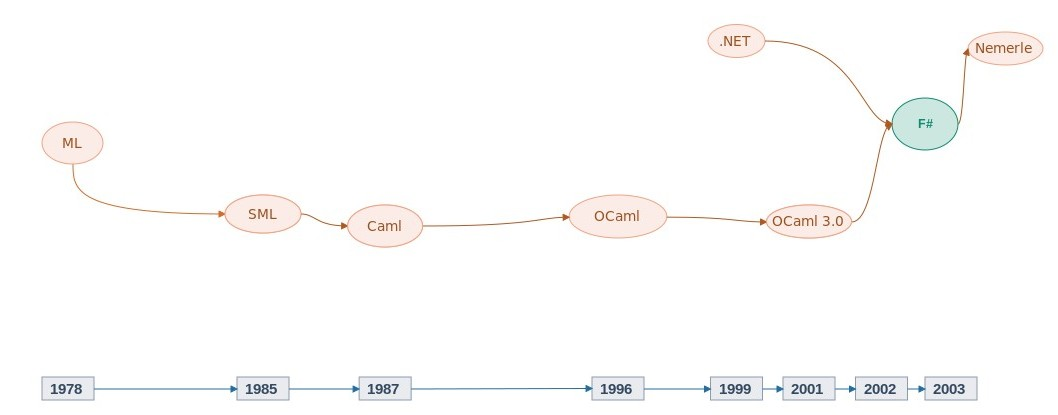
\includegraphics[scale=0.255]{stablo.jpg}
\end{center}
\caption{Razvojno stablo}
\label{fig:stablo}
\end{figure}

\section{Primena i mogućnosti}
\label{sec:primena}

Snaga F\# programskog jezika leži u svedenoj sintaksi koja omogućava laku čitljivost koda, kao i efikasan razvoj programa koji zahtevaju primenu složenih matematičkih algoritama. Jezik omogućava brzo generisanje prototipova i njihovu brzu transformaciju u produkcioni kôd. Kôd napisan u F\#-u lako se može paralelizovati, što je posebno značajno danas kada svi novi računari imaju više jezgara. F\# danas ima široku primenu u obradi baza podataka, finansijskog modelovanja, statistici i bioinformatici. Takodje, domen primene svakodnevno raste.

F\# je jezik koji ima pretežno funkcionalne karakteristike, ali on je svoju primenu pronašao u još mnogo vrsta programiranja. Neki od njih su: imperativno, objektno-orjentisano, paralelno, distribuirano, asinhrono, meta programiranje, veb programiranje, skript programiranje, analitičko programiranje, i sl. Danas se on može koristiti na velikom broju sistema, kao što su: Linux, MAC, Windows, Android, iOS, i sl. O ovome će biti više reči u nastavku. 


\section{Osnovne osobine programskog jezika F\#}

Neke od osnovnih osobina programskog jezika F\# su:\\

	$\bullet$ \textbf{Bezbedan}: F\# programi se temeljno proveravaju pre izvršenja, što ga čini bezbednim za pokretanje.

	$\bullet$ \textbf{Funkcionalan}: Funkcije mogu biti ugnježdene, prosleđene kao argumenti drugim funkcijama i vraćene kao povratna vrednost.

	$\bullet$ \textbf{Strogo tipiziran}: Provera tipova se vrši u toku kompilacije, kako bi se utvrdilo da su dobro definisani. 

	$\bullet$ \textbf{Automatski zaključuje tipove}: Tipovi vrednosti se automatski zaključuju prilikom kompilacije u zavisnosti od konteksta u kome se javljaju, što dovodi do toga da se eksplicitno navođenje retko dešava.

	$\bullet$ \textbf{Kompatibilan}: F\# programi mogu da pozivaju i da budu pozvani iz drugih programa koji su napisani na nekom od jezika koje podržava .NET platforma, kao na primer C\#\cite{microsoft_c}. 
\\
%Nešto više o njima\cite{Harrop:2008:FS:1481410}.
 
	Još neke specifičnosti jezika: \\
	
	$\bullet$ Za razliku od drugih programskih jezika struktura \textbf{if/elif/else} u svakoj grani ima povratnu vrednost.
	 
	$\bullet$ Povratna vrednost ne mora uvek biti vraćena ključnom reči \textbf{return}. Ukoliko je return izostavljen, kao povratna vrednost se uzima poslednja izvršena naredba.
	 
	$\bullet$ Korišćenjem ključne reči \textbf{let} definišemo promenljive koje se ne mogu menjati što kôd čini sigurnijim od slučajnih promena. Ukoliko smo sigurni da će se vrednost promenljive menjati, uz let se dodaje ključna reč \textbf{mutable}.
	 
	$\bullet$ Struktura \textbf{switch/case} je u F\# zamenjena {\em pattern matching}-om\cite{expertFS}.
	 
$\bullet$ Pored uobičajenih tipova podataka podržanih u većini programskih jezika, F\# podržava novi tip \textbf{option type}, koji označava vrednost promenljive koja može da postoji a i ne mora. Dve moguće vrednosti ovog tipa su: {\em Some(x)} i {\em None}.

\section{Funkcionalno programiranje}


Kao glavna, funkcionalna paradigma programskog jezika F\# podržava osnovne koncepte koji su podržani i od strane nekih drugih programskih jezika. U ovom odeljku nećemo davati prevelik značaj osnovama funkcionalne paradigme, već ćemo akcenat staviti na {\em pattern matching} \cite{expertFS}.

Jedan od važnih mehanizama u F\# programiranju jeste pattern matching. Predstavlja se kao {\em match ... with ...} konstrukcija koja kombinuje mehanizme dekompozicije i kontrole toka za poklapanje obrazaca. Kao takav, možemo ga koristiti sa  jednostavnim kolekcijama (na primer: {\em list,tuple}) i {\em option} vrednostima. Naredni listing \ref{primer} pokazuje kako se definiše pattern matching.
\\
\begin{lstlisting}[caption={Primer pattern matching-a \cite{expertFS}},frame=single, label=primer]
let urlFilter url agent =
 match (url,agent) with
 | "http://www.matf.bg.ac.rs", 99 -> true
 | "http://www.fsharp.org" , _ -> false
 | _, 86 -> true
 | _ -> false
\end{lstlisting} 

Izvedeni tip funkcije je: \\

\begin{lstlisting}
val urlFilter: string -> int -> bool
\end{lstlisting}

Izraz nakon ključne reči {\em match} je tuple tipa {\em (string * int)}. Svako pravilo obrasca se uvodi sa simbolom | iza koga sledi pravilo. Nakon navođenja pravila sledi simbol -> nakon čega sledi rezultat. Kada se izvrše, pravila obrasca se koriste jedan po jedan i prvi obrazac koji je poklopljen određuje rezultat. Prvi obrazac se poklapa ukoliko su navedene identične vrednosti, dok poslednja tri, na mestima gde se javlja simbol $\_$ za ulazne parametre, mogu da imaju bilo koju vrednost. U tabeli \ref{tab:tabela1} ćemo prikazati koje vrste obrazaca postoje u F\# i na koji način ih možemo formirati.
 
\begin{table}[h!]
\begin{center}
\caption{Načini formiranja obrazaca u F\#}
\begin{tabular}{|c|c|c|} \hline
\textbf{Opšti oblik}& \textbf{Vrsta}& \textbf{Primer}\\ \hline
(pat, ... ,pat) &Tuple pattern&(1,2,("3",x))
\\ \hline
[pat, ... ,pat] &List pattern&[x;y;z]\\ \hline
[|pat, ... ,pat|] &Array pattern&['a';'b';'c']\\ \hline
null &Null test pattern&null\\ \hline
\end{tabular}
\label{tab:tabela1}
\end{center}
\end{table}


\section{Asinhrono i paralelno programiranje}

Razlog zbog kojeg izučavamo asinhrono i paralelno programiranje se ogleda u maksimalnoj iskorišćenosti hardvera. Ranije se ovaj način programiranja izbegavao zbog dodatne složenosti i rizika od bagova. Sa pojavom velikog broja biblioteka u kombinaciji sa funkcionalnim programiranjem i izbegavanjem bočnih efekata ovaj problem je smanjen. Fokus ćemo staviti na to kako ubrzati računanje u F\# koristeći asinhrono i paralelno programiranje. Izvršavanje koda se odvija pomoću niti i F\# biblioteka. Mogu se potpuno iskoristiti prednosti više procesora i jezgara tako što se podeli jedan posao na više manjih. Najvažniji razlog uvođenja ova dva načina programiranja je ubrzanje izvršavanja programa.


\subsection{Asinhrono programiranje} 

Opisuje programe i operacije koje se izvršavaju u pozadini i završavaju nakon nekog vremena (na primer: preuzimanje novog email-a bez čestog proveravanja). Asinhroni programi na .NET platformi su pisani korišćenjem modela asinhronog programiranja (APM) \cite{apm}. APM je obrazac koji deli asinhrone operacije na dve metode: {\em BeginOperation} i {\em EndOperation}. Kada se pozove {\em BeginOperation} operacije počinju sa asinhronim izvršavanjem koje po završetku pozivaju {\em EndOperation} koji dohvata rezultat asinhronog izračunavanja. Problemi koji nastaju korišćenjem ovog obrasca su: \\

$\bullet$ Izostavljanjem poziva {\em EndOperation} dolazi do neželjenih efekata i curenja memorije. 
 
$\bullet$ Ukoliko se nekoliko asinhronih izračunavanja vrati nazad teško je pratiti tok programa.
	
$\bullet$ Posledica prethodnog problema uzrokuje pojavu špageti programiranja. \\

Umesto APM-a sve asinhrone operacije mogu se izvršavati pomoću F\# biblioteke asinhronih radnih tokova \cite{progFs}. Ključna reč {\em async} se koristi za kreiranje bloka u koji se smešta kôd za izvršavanje korišćenjem {\em let!} i {\em do!} operatora. Rezultat ovog izvršavanja će biti tipa {\em Async<T>} \cite{progFs}.

\subsection{Paralelno programiranje}

Paralelno programiranje se koristi za podelu poslova na n delova kako bi se dobilo n puta brže izvršavanje, što je retko u praksi. Najjednostavniji način korišćenja paralelnog programiranja na .NET 4.0 platformi se zasniva na upotrebi {\em Parallel Extesions} biblioteke (PFX) \cite{progFs}. Jedna od pogodnosti PFX biblioteke je ta što programer ne mora da misli o kontroli rada niti. Za razliku od paralelnog, asinhroni tok izvršavanja je dostupan i na prethodnim verzijama .NET platforme. {\em Task} objekat predstavlja osnovnu strukturu PFX paralelizma, koji ima zadatak da izvrši posao nakon nekog vremena. Kao takav, nije dovoljan za paralelne aplikacije. Zbog problema koji se javlja pri radu Task objekta sa deljivim podacima uvodi se zaključavanje podatka (eng.~{\em exclusive lock}). PFX biblioteka uvodi nove tipove kolekcija {\em System.Collections.Concurrent} \cite{sysCC} kao rešenje prethodnog problema.  


\section{Radni okviri}

Najpoznatiji i najznačajniji radni okvir (eng.~{\em framework}) za ovaj programski jezik je .NET koji je ranije već pomenut. .NET je pojednostavio razvoj RP({\em Reactive Programming}) \cite{RPapp} aplikacija. Ovaj radni okvir je potpuno besplatan i na njemu je moguće kreirati veliki broj različitih aplikacija. On podržava veliki broj programskih jezika iz različitih paradigmi, editora i biblioteka za izgradnju mobilnih i veb aplikacija. Razvijene su dve glavne komponente za korišćenje rekurzivnog paralelnog izračunavanja na lokalnoj mreži i obe su dostupne programima na .NET platformi \cite{ppNETframework}. 

Temelj .NET platforme je zajednička jezička infrastruktura CLI ({\em Common Language Infrastructure}) \cite{cli}. Pokretanje F\# koda na ovoj platformi se vrši tako što na samom početku kompajler prevodi kôd u binarni fajl koji je preveden na asemblerski jezik višeg nivoa koji se zove MSIL ({\em Microsoft Intermediate Language}) \cite{msil}. Implementacija na CLI kompajleru ovog asemblerskog koda u toku izvršavanja je mnogo brža nego da je kôd samo interpretiran i ova kompilacija se izvršava u trenutku \cite{progFs}.
Kôd koji je preveden u MSIL i izvršen u trenutku, predstavlja kôd za upravljanje za razliku od kodova pisanih na drugim programskim jezicima kao što su C ili C++.   

Postoje neke prednosti za prolazak kroz CLI ili upravljani kôd, a ne direktnog kompiliranja na mašinski nivo:	\\

	$\bullet$ kompatibilnost medju jezicima
	
	$\bullet$ mogućnost rada na više platformi
	
	$\bullet$ mašinska nezavisnost
\\

.NET platforma ima još jednu prednost, a to je prikupljanje smeća što omogućava programeru da ne razmišlja mnogo o alociranju i oslobađanju memorije, već da se samo skoncentriše na pisanje koda. Iako ne mora da obraća pažnju na smeće i rad sa memorijom poželjno je da programer zna na koji način taj sakupljač smeća radi, kako on oslobađa memoriju i rešava taj problem.

Naravno da ova platforma nije jedina koja se koristi za ovaj programski jezik, pored nje postoje: veb radni okviri (na primer: {\em Suave, Fable, ASP.NET Core, Giraffe, WebSharper, Freya, NancyFx, Serving Requests with IHttpHandler, Serving Requests with Azure, Functions, Pure F\# Web API 2.0, SignalR, ServiceStack, ASP.NET Blazor}) i radni okviri za testiranje veba (na primer: {\em Web Testing, Frameworks, Canopy for Client-side Testing, Unit Testing Libraries}) \cite{fwFs}.

\section{Uputstvo za instalaciju}

U ovom poglavlju biće opisano uputstvo za instalaciju programskog jezika F\# na Windows i Linux operativnim sistemima, kao i uputstvo za pokretanje F\# programa.

\subsection{Uputstvo za Windows}

Na ovom operativnom sistemu postoje tri načina za instalaciju F\#-a. To su: {\em Visual studio} \cite{vStud}, {\em Visual Studio Code} \cite{vStudCode} i {\em JetBrains Rider} \cite{jetBrains}.

Pokretanje F\# koda na Windows-u se vrši tako što prvo označite kôd ili deo koda koji želite da se izvrši. Zatim, desnim klikom na miša izaberite opciju {\em pošalji interaktivno} (eng.~{\em send to interactive}) ukoliko je interaktivni prozor tj. prozor na kom se ispisuje rezultat otvoren ili iskoristite prečicu \textbf{Alt + Enter}.

\subsubsection{Visual studio}
	
Na Windows operativnim sistemima se uglavnom koristi {\em Visual Studio} alat. {\em Visual studio 2017} je alat koji dolazi sa podrškom za F\# u svim verzijama: {\em Professional, Enterprise} i {\em Community} (verzija je potpuno besplatna). Međutim, ukoliko imate  već instaliran {\em Visual Studio 2012/13/15  Professional} ili {\em Above} možete ga takođe koristiti zato što i on podržava alate za F\# iako nije toliko napredan kao {\em Visual Studio 2017}.

\subsubsection{Visual Studio Code}
	
{\em Visual Studio Code} je besplatna platforma koja podržava mnogo jezika, a među njima i F\#. On je podržan od strane {\em Ionide} \cite{ionide}.

\textbf{1.korak:} Instalirati {\em Visual Studio Code} za Windows.

\textbf{2.korak:} Pritisnuti \textbf{Ctrl+Shift+p} i ukucati sledeću naredbu za instalaciju {\em Ionide} paketa za {\em Visual Studio Code}:
\\
\begin{lstlisting}
 ext install Ionide-fsharp
\end{lstlisting}
 
\subsubsection{JetBrains Rider}

{\em JetBrains Rider} je platforma .NET IDE izgrađena pomoću {\em InteliJ} i {\em ReSharper} tehnologije. {\em JetBrains} nudi podršku .NET i .NET Core aplikacijama na svim platformama.

\textbf{1.korak:} Instalirati {\em JetBrains} za Windows.

\textbf{2.korak}(opciono): Instalirati poslednju vrziju .NET Core SDK.

Takođe vam je potrebno da instalirate ceo {\em Visual Studio} ili F\# kompajler.


\subsection{Uputstvo za Linux}

Kada koristite jezik koji podržava .NET platforma, kao što je F\#, onda on zahteva Mono \cite{mono} softversku platformu. Većina Linux distributera sadrži neku verziju te platforme koja omogućava programerima lakše kreiranje aplikacija. 

Instalacija F\# na Linuxu se izvršava na potpuno identičan način za {\em Ubuntu, Mint} i {\em Debian} verzije.

Za pokretanje F\# programa na Linux-u preko terminala koristi se sledeća naredba ukoliko se nalazite u direktorijumu u kom se nalazi primer koji pokrećete.
\\
\begin{lstlisting}
fsharpc primer.fs
\end{lstlisting}

\subsubsection{Ubuntu/Mint/Debian}

\textbf{1.korak:} Dodati {\em Mono} \cite{mono} repozitorijum vašem menadžeru paketa.

\textbf{2.korak:} Instalirati F\# koji će istovremeno povući novu verziju {\em Mono}-a ukoliko je to potrebno.
\\
\begin{lstlisting}
sudo apt-get update
sudo apt-get install fsharp
\end{lstlisting}
 
\section{Fizz Buzz problem}
\textit{Fizz Buzz} je problem koji je osmišljen za intervjuisanje kandidata koji konkurišu za posao programera. Treba napisati program koji štampa brojeve od 1 do 100 pri čemu, ako je broj deljiv sa 3 tada umesto tog broja ispisuje \textit{Fizz}, ako je deljiv sa 5 ispisuje \textit{Buzz}, dok ako je deljiv i sa 3 i sa 5 ispisuje \textit{FizzBuzz}. \\

\begin{lstlisting}[caption={Fizz Buzz \cite{fizzBuzz}},frame=single, label=fizzbuzz]
let (|Fizz|Buzz|FizzBuzz|Other|) n =
    match (n % 3, n % 5) with
    | 0, 0 -> FizzBuzz
    | 0, _ -> Fizz
    | _, 0 -> Buzz
    | _ -> Other n

let fizzBuzz =
    function
    | Fizz -> "Fizz"
    | Buzz -> "Buzz"
    | FizzBuzz -> "FizzBuzz"
    | Other n -> n.ToString()

seq { 1..100 } |> Seq.map fizzBuzz|> Seq.iter (printfn "%s")
\end{lstlisting}

Navedeni primer \ref{fizzbuzz} sadrži korisničko definisani šablon koji prepoznaje četiri moguća obrasca. Obrazac je dat u obliku para (eng.~{\em tuple}) pri čemu je četvrti obrazac \textit{wildcard} i vraća \textit{Other} zajedno sa brojem koji odgovara tom obrascu. Šablon dalje koristimo u \textit{pattern matching} izrazu koji nam vraća niske za ispis. Na kraju sprovodimo sekvencu od 1 do 100 kroz \textit{Seq.map} koja primenjuje \textit{pattern matching} nad svakim elementom date sekvence i zamenjuje ga odgovarajućom niskom. Konačno, funkcija \textit{Seq.iter} iterira kroz sekvencu i ispisuje rezultat.

\section{Jedinica mere - osobina svojstvena jeziku F\texttt{\#}}
Jedinica mere (eng.~{\em Units of Measure}), svojstvena samo za F\#, je mehanizam koji omogućava da se numeričkim tipovima pridruže dodatne informacije i na taj način spreče potencijalne greške pri radu sa različitim mernim jedinicama \cite{unitsOfMeasure}. U nastavku je dat demonstrativni program \ref{jedinice} koji računa godišnju zaradu u evrima. \\

\begin{lstlisting}[caption={Primer jedinice mere \cite{unitsOfMeasureExample}},frame=single, label=jedinice]
[<Measure>] type rsd
[<Measure>] type eur
[<Measure>] type hour
[<Measure>] type week
[<Measure>] type year

let hoursBilledPerWeek = 40.0<hour/week>
let weeksWorkedPerYear = 35.0<week/year>
let rsdPerHour = 1000.0<rsd/hour>
let exchangeRate = 0.008547<eur/rsd>

let eurPerYear = rsdPerHour * hoursBilledPerWeek * weeksWorkedPerYear * exchangeRate

let bonus = 500.0<eur/year>

printfn "%f" (eurPerYear + bonus)

// Output: 12465.8

\end{lstlisting}

Jedinica mere se definiše kao \textbf{[<Measure>] type} nakon čega sledi njen naziv. U našem primeru imamo vremenske jedinice (sat, vikend i godina) kao i jedinice koje označavaju valutu (dinar i evro). Dalje, pri definisanju promenljivih, dodatno pišemo informaciju o jedinici. Zbog toga, ako definišemo zaradu po satu dopisujemo \textbf{<rsd/hour>}. Program na kraju ispisuje zaradu sa godišnjim bonusom. 

Ukoliko bi promenili 10. liniju koda i stavili suprotan odnos valuta \ref{valuta}, tj. vrednost evra u odnosu na dinar, došlo bi do greške u fazi kompilacije \ref{greska}. \\
 
\begin{lstlisting}[caption={Promenjen odnos valuta},frame=single, firstnumber=10, label = valuta]
let exchangeRate = 117.0<rsd/eur>
\end{lstlisting}
\begin{lstlisting}[caption={Kompajler prepoznaje grešku},frame=single, label=greska]
Error: The unit of measure 'eur/year' does not match the unit of measure 'rsd ^ 2/(eur year)'
\end{lstlisting}

Daljom proverom vidimo da, ako na ovaj način definišemo odnos valuta, moramo da izmenimo formulu. Ukoliko u 12. liniji koda \ref{12linija}, umesto što množimo sa kursnom razlikom, podelimo sa istom, kompajler se više neće buniti i dobićemo validnu vrednost. \\

\begin{lstlisting}[caption={Ispravljena linija},frame=single, firstnumber=12,label={12linija}]
let eurPerYear = rsdPerHour * hoursBilledPerWeek * weeksWorkedPerYear / exchangeRate
\end{lstlisting}

\section{Zaključak}
\label{sec:zakljucak}

Već nekoliko puta smo naglasili da je F\# jezik velikih mogućnosti. Ovim radom predstavili smo neke zanimljive koncepte koje on poseduje, ali se nismo bavili osnovama koje mogu pomoći u učenju ovog jezika. Ako smo uspeli da zaintrigiramo čitaoca, savetujemo učenje jezika ili unapređivanje znanja o njemu ukoliko se već susretao sa njim i ranije. Rad nije bio namenjen tome. U literaturi koju smo koristili postoji mnogo knjiga, članaka i sajtova na ovu temu koji u učenju mogu pomoći. Objasnili smo kako se na dva sistema mogu pokrenuti platforme za rad u F\#-u. Osim toga, postoji još puno lako dostupne literature na slične teme.

\addcontentsline{toc}{section}{Literatura}
\appendix
\bibliography{seminarski} 
\bibliographystyle{plain}


\end{document}